%In this section, \textbf{we address the consistency models usually adopted by} distributed storage systems.
%we present the concepts of the consistency models in distributed storage systems.
%\textbf{First, we highlight the consistency perspectives} in this environment, and then we provide a hierarchical overview of the main consistency models.

%\subsection{Perspectives on Consistency}
%\subsection{Consistency Perspectives}

{\al A consistency model may be defined as a contract between a data storage system and the data processes that access it~\cite{tanenbaum:2007}. It defines strategies for supporting consistency within a distributed data storage system. However, trade-offs due to the CAP theorem require the choice from a range of models to address different consistency levels}, which may vary from a relaxed model to a strict one~\cite{bermbach2013consistency}. {\al In this context, there are two distinct perspectives to be considered in a distributed data storage system with respect to consistency}~\cite{tanenbaum:2007}: the \textit{data provider} and the {\al \textit{clients}}.
%In this context, there are two perspectives \textbf{in terms of consistency} to be considered in a distributed storage system \cite{tanenbaum:2007}: the \textit{provider} and the \textit{client}.
%demanding of the systems the need to incorporate a range of models that address consistency guarantees that varying from a relaxed consistency model to a strict consistency model \cite{bermbach2013consistency}. In this context, there are two perspectives to be considered on consistency in a distributed storage system \cite{tanenbaum:2007}: the provider and the client.

From the perspective of the data provider, the operations from all processes that want to access the data must be synchronized and ordered to guarantee correct results. From the perspective of the clients, it is often the case that shared updates are rare and they mostly access their private data. In that case, their major concern is that their own operations are consistent, what may be simpler to achieve.
%
%{\al The provider is responsible for synchronizing the processes {\dg that want to access} the replicas and ordering their operations.}
%%the synchronization processes among the replicas and the ordering of the operations. 
%The other perspective refers to the process of interaction between the client and the storage system. 
These two {\al consistency perspectives} are called \textit{data-centric} and \textit{client-centric}~\cite{tanenbaum:2007}. Next, we discuss the consistency models related to each {\al perspective}.
\vspace{2mm}

\subsection{Data-centric Consistency Models}
In this perspective, the consistency models seek to ensure that the data access process follows certain rules so that the storage system can work correctly. These rules are based on the definition of the results that are expected after read and write operations, even considering that these operations are concurrently performed. However, the absence of a global clock makes {\al the identification} of the last write operation a difficult task, %so that alternatively, it is required to apply 
which requires some restrictions on the data values that can be returned by a read operation, thus leading to a range of consistency models~\cite{tanenbaum:2007}.

The {\al consistency models that fall in this category %related to this perspective 
are:} \textit{weak consistency, PRAM consistency, causal consistency, sequential consistency and strict consistency}. 
%{\dg which are discussed next.} %{\rc  We describe each one of these models next}.
\vspace{1mm}

\subsubsection{Weak Consistency}

The weak consistency model offers the lowest possible ordering guarantee. As this guarantee is very weak, 
%it makes sense to affirm 
we can say that
it does not really exist, since an implementation may or may not have a protocol to synchronize replicas. It provides consistency to a group of transactions instead of to individual reads and writes, which is done by {\dg the} stricter consistency models 
{\dg that follow next} (PRAM, causal and sequential)~\cite{tanenbaum:2007, Vogels:2009}. % described next.
\vspace{1mm}

\subsubsection{PRAM Consistency}
 
PRAM (Pipelined Random Access Memory) consistency, also known as FIFO consistency, is a model in which write operations from a single process are seen by other processes in the same order that they were issued by its original process, whereas writes from different processes may be seen in a different order {\al by} different processes. In other words, there is no guarantee on the order in which the writes are seen by different processes, although writes from a single source must %arrive in order,
keep their order as if they were in a pipeline~\cite{lipton1988pram, tanenbaum:2007}.
\vspace{1mm}

\subsubsection{Causal Consistency}

Causal consistency is a model in which a sequential ordering is always maintained only between requests that have a causal relationship. Thus, concurrent requests do not share this relationship. In this case, all requests must be serialized in the same order on all replicas \cite{tanenbaum:2007}. {\al Thus, in a scenario of an always-available storage system in which requests have causal dependencies, a consistency level stricter than that provided by the casual model} cannot be achieved due to trade-offs of the CAP theorem~\cite{mahajan2011consistency}.

{\al More specifically,} two requests have a causal dependency if at least one of the following two conditions is achieved: (1) both requests are executed on a single thread and the execution of one precedes the other in time; (2) if a request B reads a value that has been written by a request A. Moreover, the relationship is transitive, so if A and B have a causal relation, and B and C also have a causal relation, then A and C share the same relationship~\cite{tanenbaum:2007, Vogels:2009}.
\vspace{1mm}

\subsubsection{Sequential Consistency}

Sequential consistency is a stricter  model that differs from the previous one in the sense that it extends to all requests %in order that 
the need of the replicas to agree on the ordering of non-causally related requests. It requires  that all operations be serialized in the same order on all replicas and that those related to the same process are executed in the order that they are received by the storage system~\cite{tanenbaum:2007}
%{\rc This model requires that the same serialization order imposed by the requests (verificar esta desri\c{c}\~ao)} is maintained on all replicas and the storage system must execute the requests in the order that they are received if they were sent by the same client~\cite{tanenbaum:2007}.
%\vspace{2mm}

\subsubsection{Strict Consistency}

Strict consistency is the model that provides the strongest consistency level. It states that if a write operation is performed on a data item, the result needs to be instantaneously visible to all processes, regardless in which replica the operation has occurred. To achieve this, an absolute global time order must be maintained~\cite{tanenbaum:2007}.
\\
%\vspace{3mm}

\subsection{Client-centric Consistency Models}

In this perspective, the distributed data store is characterized by an relative absence of simultaneous updates.
Also, when a simultaneous update occurs, the solution of any concurrency problem is simple to achieve.
%{\al Thus, in case that updates occur, there is no need to resolve them.}
%there are no problems in resolve them. 
The emphasis is then to maintain a consistent view of data items for an individual client process that is currently operating on the data store~\cite{tanenbaum:2007}. 
The models in this category are: \textit{eventual consistency, monotonic reads consistency, monotonic writes consistency, read-your-writes consistency} and \textit{writes-follow-reads consistency}. %{\rc We describe each one of these consistency models next.}
%\vspace{1mm}

\subsubsection{Eventual Consistency}

The eventual consistency model states that all updates will propagate through the system and all replicas will gradually become consistent in the case of the absence of updates for a long time \cite{tanenbaum:2007, Vogels:2009}. Although this model does not provide concrete consistency guarantees, there are several distributed storage systems that implement it~\cite{Chang06bigtable:a, decandia2007dynamo, Ghemawat2003Google, lakshman2010cassandra}.
\vspace{1mm}

\subsubsection{Monotonic Read Consistency}

The monotonic read consistency model guarantees that if a process reads a version of a data item \textit{d} at time \textit{t}, it will never see an older version of \textit{d} at a later time. In an scenario where data visibility is not guaranteed to be instantaneous, at least the versions of a data item will become visible in chronological order \cite{tanenbaum:2007, Vogels:2009}.
\vspace{1mm}

\subsubsection{Monotonic Write Consistency}

The monotonic write consistency model guarantees that a data store must serialize two writes \textit{$w_{1}$} and \textit{$w_{2}$} in the same order that they were sent by the same client~\cite{tanenbaum:2007, Vogels:2009}. For instance, if the initial write operation \textit{$w_{1}$} is lost, it is not allowed to the subsequent write \textit{$w_{2}$} to overwrite that data item.
\vspace{1mm}

\subsubsection{Read-Your-Writes Consistency}

Read-your-writes consistency is closely related to the monotonic reads model. It guarantees that once a write operation is performed on a data item \textit{d}, its effect will be seen by any successive read operation performed on \textit{d} by the same process~\cite{tanenbaum:2007, Vogels:2009}. This means that if a client has written a version \textit{v} of a data item \textit{d}, it will always be able to read a version at least as new as \textit{v}. 
%or upper.
\vspace{1mm}

\subsubsection{Writes-Follow-Reads Consistency}

Writes-follow-reads consistency guarantees that if a write operation \textit{w} is requested by a process on a data item \textit{d}, but there has been a previous read operation on \textit{d} by the same process, then it is guaranteed that \textit{w} will only be executed on the same or on a more recent value of \textit{d} previously read~\cite{tanenbaum:2007}.
\vspace{3mm}


\subsection{Hierarchical View of the Consistency \\ Models}
%https://www.overleaf.com/8967554ryqqdyzyrdcp#
In order to achieve a better understanding of the relationships among the consistency models, they can be hierarchically organized according to their degree of strictness from a lower consistency level to a higher one (see Figure~\ref{fig:hierarchicalView}).  

\begin{figure}[h]
\centering	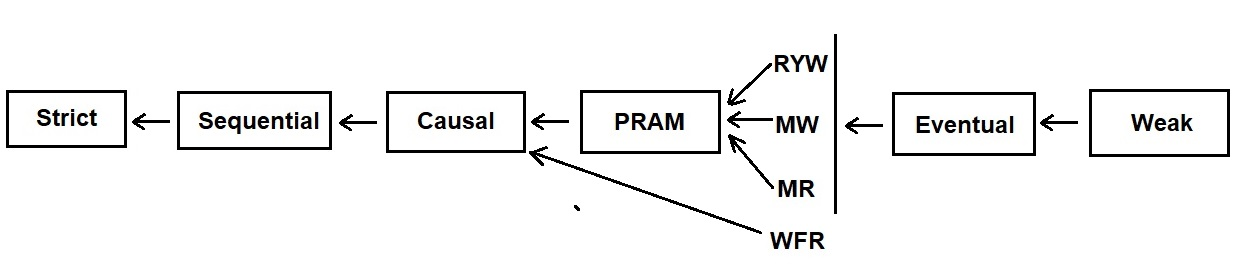
\includegraphics[width=0.48\textwidth]{fig2b.jpg}

\vspace{-3mm}
\caption{Hierarchical View of the Consistency Models.}
\label{fig:hierarchicalView}
\end{figure}
%\vspace{-1mm}

This hierarchical organization also considers some model combinations, such as the PRAM consistency model that may be seen as a combination of the monotonic read (MR), monotonic write (MW) and read-your-writes (RYW) models~\cite{bailis2013highly}. In addition, according to Brzezi\'nski et al.~\cite{brzezinski2004session}, there is also a relationship between causal consistency, which is a data-centric model, and the client-centric perspective,  
%and apparently, 
thus meaning that causal consistency is similar to write-follows-reads (WFR). 
%\vspace{2mm}
\\

\begin{comment}

\begin{figure}[h]
\centering
\begin{minipage}{18cm}
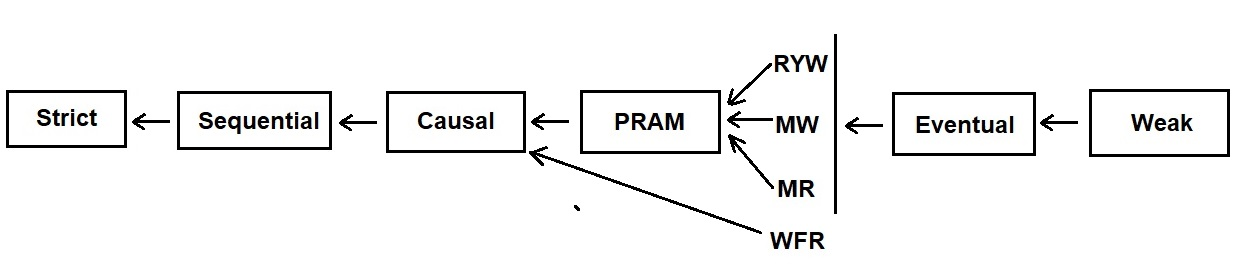
\includegraphics[width=0.43\textwidth]{fig2b.jpg}
\label{fig:fig2b}
\end{minipage}
\caption{Hierarchy of the Consistency Models}
\end{figure}
\end{comment}